Como na secção anterior, apresenta-se de seguida os resultados obtidos para um sinal sinusoidal de $25$Hz, $5$V de amplitude e $0$V de \textit{offset}, para a variação de uma fonte DC (escala de $5$V/div como pedido) e ainda uma onda quadrada de $60$Hz, $4$V de amplitude e $-1$V de \textit{offset}. Agora com o ajuste experimental, comentam-se as linhas \texttt{73}, \texttt{74} e \texttt{75} e descomenta-se a linha \texttt{76} da função \texttt{read\_and\_calculate()}.

\vspace{1.5cm}

\begin{figure}[H]
    \centering
    \begin{subfigure}{0.35\textwidth}
        \centering
        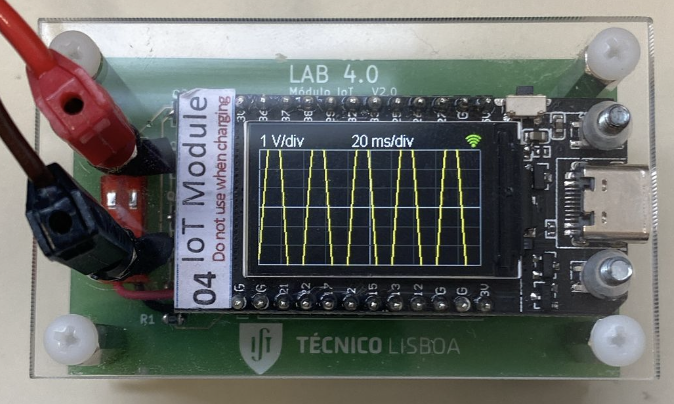
\includegraphics[width=1\linewidth]{Imagens/Testes no laboratório/Calibrado/Vertical 1V.png}
        \captionsetup{justification=centering}
        \caption{1V/div e 20ms/div}
        \label{fig:1V/div e 20ms/div calibrado}
    \end{subfigure}
    \begin{subfigure}{0.35\textwidth}
        \centering
        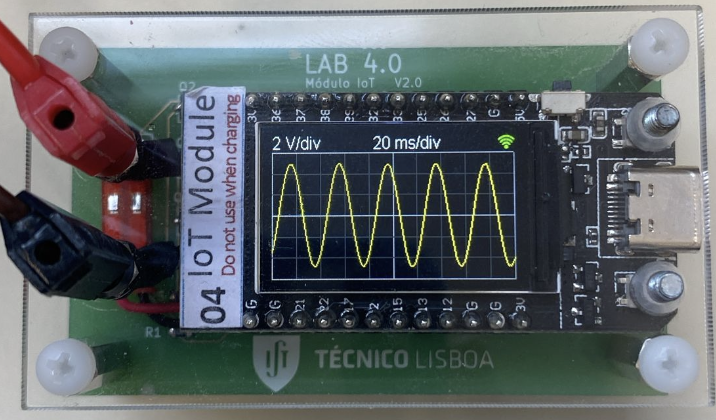
\includegraphics[width=1\linewidth]{Imagens/Testes no laboratório/Calibrado/Vertical 2V.png}
        \captionsetup{justification=centering}
        \caption{2V/div e 20ms/div}
        \label{fig:2V/div e 20ms/div calibrado}
    \end{subfigure}
    \begin{subfigure}{0.35\textwidth}
        \centering
        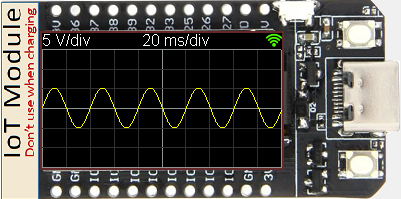
\includegraphics[width=1\linewidth]{Imagens/Testes no laboratório/Calibrado/Vertical 5V.png}
        \captionsetup{justification=centering}
        \caption{5V/div e 20ms/div}
        \label{fig:5V/div e 20ms/div calibrado}
    \end{subfigure}
    \begin{subfigure}{0.35\textwidth}
        \centering
        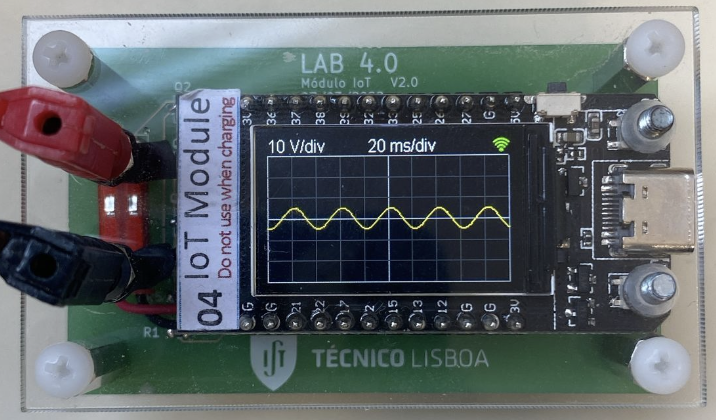
\includegraphics[width=1\linewidth]{Imagens/Testes no laboratório/Calibrado/Vertical 10V.png}
        \captionsetup{justification=centering}
        \caption{10V/div e 20ms/div}
        \label{fig:10V/div e 20ms/div vertical calibrado}
    \end{subfigure}
    \captionsetup{justification=centering}
    \caption{Variação da escala vertical (calibrado)}
    \label{fig:Variação da escala vertical (calibrado)}
\end{figure}

\begin{figure}[H]
    \centering
    \begin{subfigure}{0.35\textwidth}
        \centering
        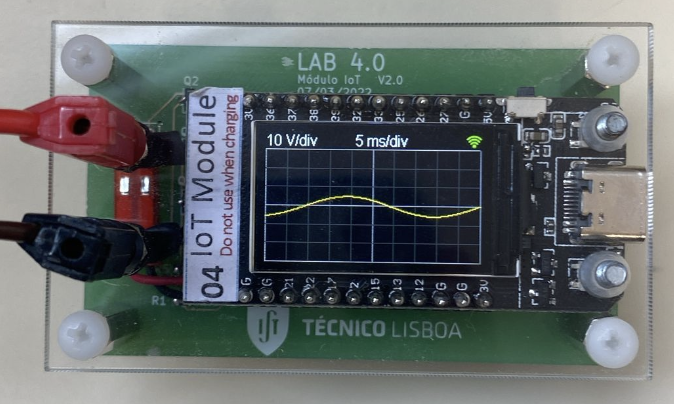
\includegraphics[width=1\linewidth]{Imagens/Testes no laboratório/Calibrado/Horizontal 5ms.png}
        \captionsetup{justification=centering}
        \caption{10V/div e 5ms/div}
        \label{fig:10V/div e 5ms/div calibrado}
    \end{subfigure}
    \begin{subfigure}{0.35\textwidth}
        \centering
        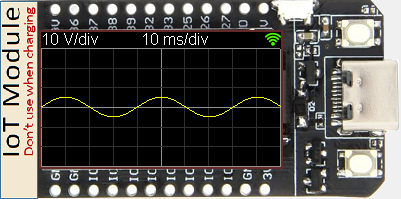
\includegraphics[width=1\linewidth]{Imagens/Testes no laboratório/Calibrado/Horizontal 10ms.png}
        \captionsetup{justification=centering}
        \caption{10V/div e 10ms/div}
        \label{fig:10V/div e 10ms/div calibrado}
    \end{subfigure}
\end{figure}

\begin{figure}[H]\ContinuedFloat
    \centering
    \begin{subfigure}{0.35\textwidth}
        \centering
        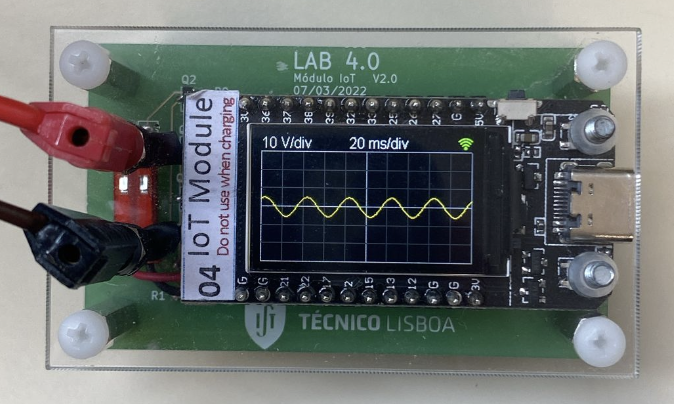
\includegraphics[width=1\linewidth]{Imagens/Testes no laboratório/Calibrado/Horizontal 20ms.png}
        \captionsetup{justification=centering}
        \caption{10V/div e 20ms/div}
        \label{fig:10V/div e 20ms/div horizontal calibrado}
    \end{subfigure}
    \begin{subfigure}{0.35\textwidth}
        \centering
        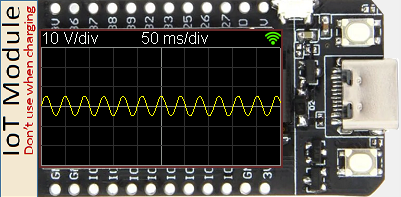
\includegraphics[width=1\linewidth]{Imagens/Testes no laboratório/Calibrado/Horizontal 50ms.png}
        \captionsetup{justification=centering}
        \caption{10V/div e 50ms/div}
        \label{fig:10V/div e 50ms/div calibrado}
    \end{subfigure}
    \captionsetup{justification=centering}
    \caption{Variação da escala horizontal (calibrado)}
    \label{fig:Variação da escala horizontal (calibrado)}
\end{figure}

\vspace{-0.4cm}

\begin{figure}[H]
    \centering
    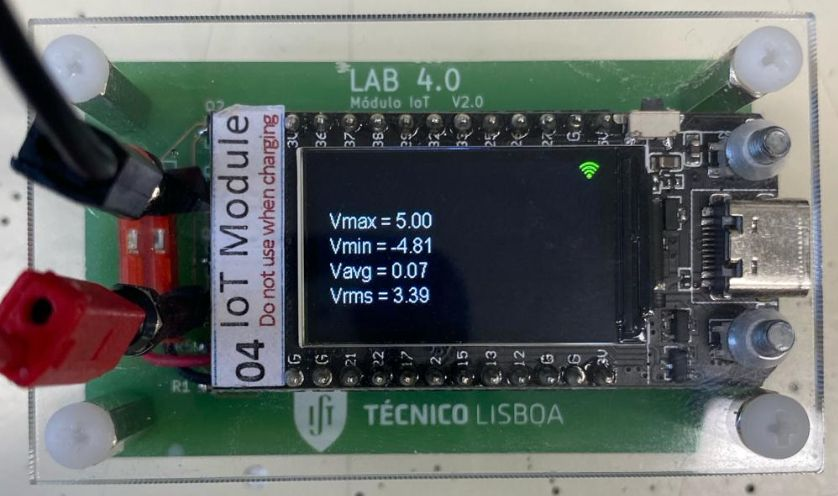
\includegraphics[width=0.35\textwidth]{Imagens/Testes no laboratório/Calibrado/Botão 13.jpeg}
    \captionsetup{justification=centering}
    \caption{Funcionamento do duplo clique do botão 1 (calibrado)}
    \label{fig:Funcionamento do duplo clique do botão 1 (calibrado)}
\end{figure}

\vspace{-0.4cm}

\begin{figure}[H]
    \centering
    \begin{subfigure}{0.35\textwidth}
        \centering
        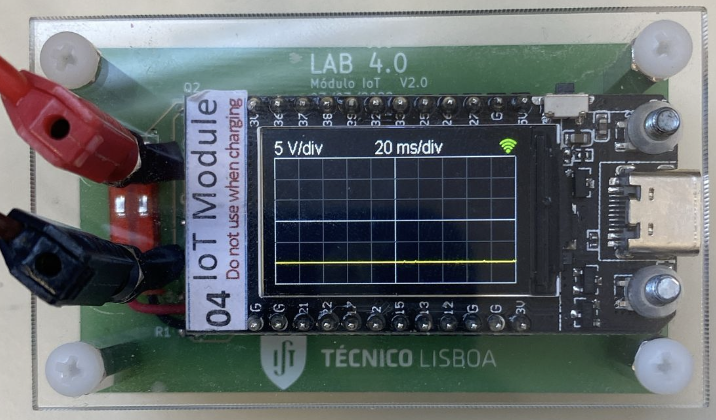
\includegraphics[width=1\linewidth]{Imagens/Testes no laboratório/Calibrado/DC -10V.png}
        \captionsetup{justification=centering}
        \caption{DC -10V}
        \label{fig:DC -10V calibrado}
    \end{subfigure}
    \begin{subfigure}{0.35\textwidth}
        \centering
        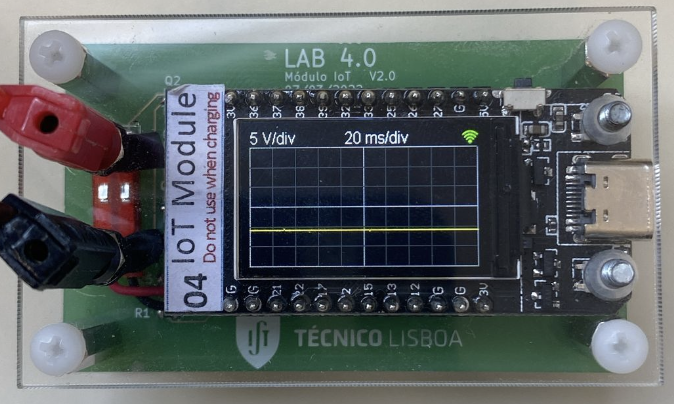
\includegraphics[width=1\linewidth]{Imagens/Testes no laboratório/Calibrado/DC -5V.png}
        \captionsetup{justification=centering}
        \caption{DC -5V}
        \label{fig:DC -5V calibrado}
    \end{subfigure}
    \begin{subfigure}{0.35\textwidth}
        \centering
        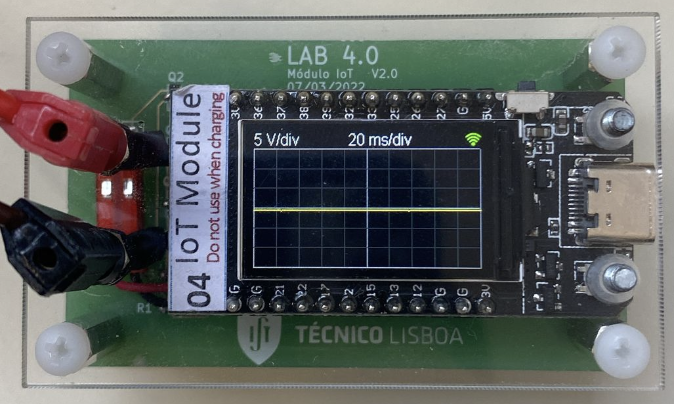
\includegraphics[width=1\linewidth]{Imagens/Testes no laboratório/Calibrado/DC 0V.png}
        \captionsetup{justification=centering}
        \caption{DC 0V}
        \label{fig:DC 0V calibrado}
    \end{subfigure}
    \begin{subfigure}{0.35\textwidth}
        \centering
        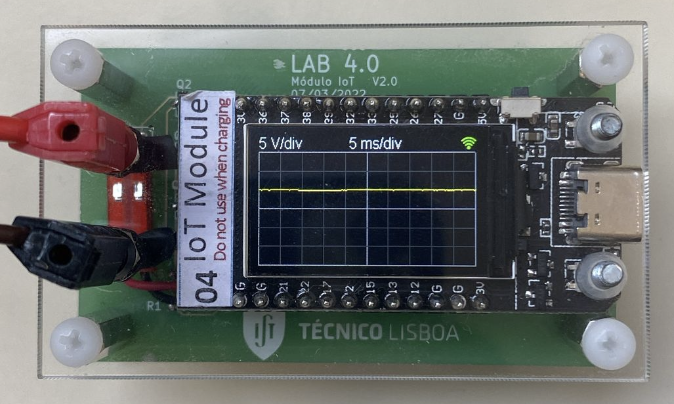
\includegraphics[width=1\linewidth]{Imagens/Testes no laboratório/Calibrado/DC 5V.png}
        \captionsetup{justification=centering}
        \caption{DC 5V}
        \label{fig:DC 5V calibrado}
    \end{subfigure}
    \begin{subfigure}{0.35\textwidth}
        \centering
        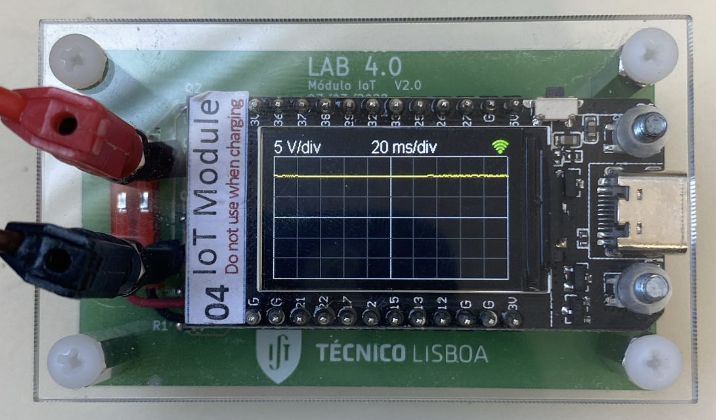
\includegraphics[width=1\linewidth]{Imagens/Testes no laboratório/Calibrado/DC 10V.png}
        \captionsetup{justification=centering}
        \caption{DC 10V}
        \label{fig:DC 10V calibrado}
    \end{subfigure}
    \captionsetup{justification=centering}
    \caption{Variação de uma tensão DC (calibrado)}
    \label{fig:Variação de uma tensão DC (calibrado)}
\end{figure}

\begin{figure}[H]
    \centering
    \begin{subfigure}{0.35\textwidth}
        \centering
        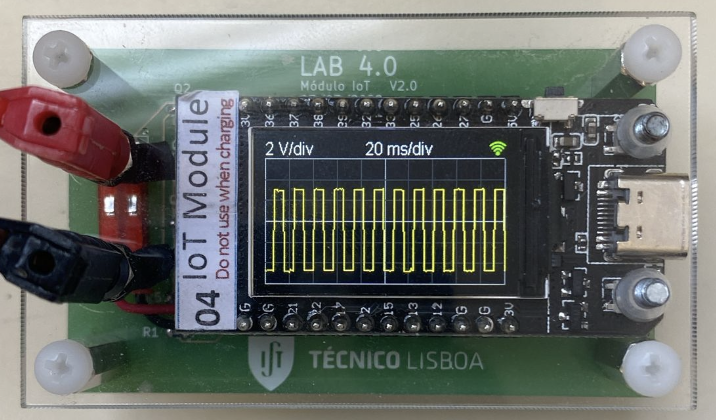
\includegraphics[width=1\linewidth]{Imagens/Testes no laboratório/Calibrado/Onda quadrada do enunciado.png}
        \captionsetup{justification=centering}
        \caption{Onda quadrada}
        \label{fig:Onda quadrada calibrado}
    \end{subfigure}
    \begin{subfigure}{0.35\textwidth}
        \centering
        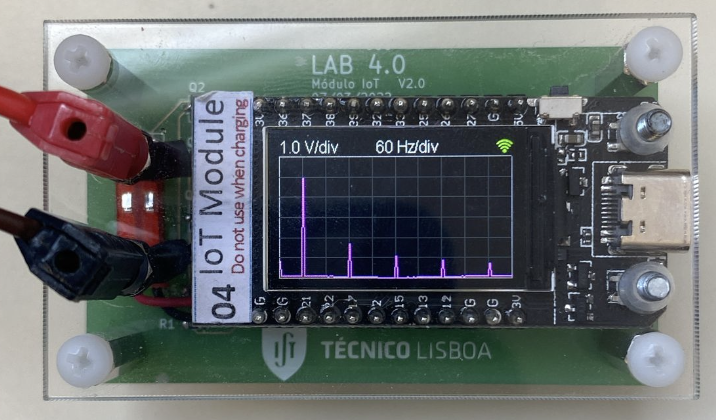
\includegraphics[width=1\linewidth]{Imagens/Testes no laboratório/Calibrado/Onda quadrada do enunciado espetro.png}
        \captionsetup{justification=centering}
        \caption{Espetro da onda quadrada}
        \label{fig:Espetro da onda quadrada calibrado}
    \end{subfigure}
    \captionsetup{justification=centering}
    \caption{Onda quadrada do enunciado e o seu espetro (calibrado)}
    \label{fig:Onda quadrada do enunciado e o seu espetro (calibrado)}
\end{figure}

Como previsto, a calibração permitiu obter representações dos sinais realmente corretas como se pode ver nas ilustrações acima apresentadas. No entanto, como dito na \nameref{sec:Introdução}, as imperfeições não são completamente aniquiladas devido às não idealidades do sistema que causam ruído (particularmente visível na \autoref{fig:Variação de uma tensão DC (calibrado)}), nomeadamente a impedância associada ao gerador de funções usado para gerar o sinal de entrada e fazer curto-circuito no módulo IoT. Pela \autoref{fig:Funcionamento do duplo clique do botão 1 (calibrado)} vemos ainda o efeito das não idealidades no cálculo de \texttt{Vmin}, uma vez que este não é o simétrico de \texttt{Vmax}. Pela \autoref{fig:Onda quadrada do enunciado e o seu espetro (calibrado)} vemos também o efeito do ruído na representação no domínio do tempo e, por sua vez, um ligeiro decréscimo do pico principal do espetro.

Desta maneira, após testes em simulação e no laboratório verifica-se o correto funcionamento do ficheiro \texttt{main.py} desenvolvido, assim como um bom ajuste experimental para o módulo IoT $04$ utilizado.
